% Document class
\documentclass[11pt,a4paper]{article}

% Some useful user-commands
\newcommand{\COMM}[1]{{\textcolor{red}{#1}}}
\newcommand{\figurebox}[3]{\resizebox{#1}{#2}{\input{figures/#3}}}
\newcommand{\graphicbox}[3]{\resizebox{#1}{#2}{\input{graphics/#3}}}
\newcommand{\imagebox}[3]{\resizebox{#1}{#2}{\includegraphics{images/#3}}}

% Include useful packages
\usepackage{amsmath}
\usepackage{amssymb}
\usepackage{amsthm} 
\usepackage{graphicx}
\usepackage{color}
\usepackage{url}
\usepackage{supertabular}
\usepackage{tabularx}
\usepackage{setspace}
\usepackage{multirow}
\usepackage{array}
\usepackage{comment}

\usepackage[left=1in, right=1in, top=1in, bottom=1in, includefoot, headheight=13.6pt]{geometry}

% Alter the intra-line and the inter-paragraph space
%\setlength{\parindent}{0pt}
%\setlength{\parskip}{1ex}
\setstretch{1.33}

% Set a more beautiful font
\usepackage{mathpazo}

% Start of the document
\begin{document}

\title{\Huge{Conditional Replenishment \\ + \\ Motion Compensation}\\\Large{Internal report}}
\date{}

\maketitle 

\section{Introducci\'on}



\section{Algoritmo}

\begin{enumerate} 

  \item Se descargan las dos primeras im\'agenes de la secuencia, $I_i$
  ($even\_image$) y $I_{i+1}$ ($odd\_image$).

  \item Calculamos los vectores de movimiento entre las dos im\'agenes. \\ 
  {\color{blue}\texttt{MCJ2K/bin/me -p 2 -x $X$ -y $Y$ -b $B$ -s $S$ -e $even\_image$ -o $odd\_image$ -a $A$ -d $D$}}

    \begin{itemize}
      \item $X$: Ancho de la imagen.
      \item $Y$: Alto de la imagen.
      \item $B$: Tama\~no de bloque $B \times B$.
      \item $S$: Tama\~no del \'area de b\'usqueda.
      \item $even\_image$: Imagen par, $I_i$.
      \item $odd\_image$: Imagen impar, $I_{i+1}$.
      \item $A$: Precisi\'on subpixel.
      \item $D$: Tama\~no del borde de los bloques.
    \end{itemize}

  \item Generamos una imagen predicci\'on a partir de la imagen $I_{i+1}$
  ($odd\_image$) y los vectores de movimiento calculados en el paso anterior. \\
  {\color{blue}\texttt{MCJ2K/bin/decorrelate -p 2 -x $X$ -y $Y$ -b $B$ -s $S$ -e $odd\_image$ -o $odd\_image$ -i motion -v $V$}}

    \begin{itemize}
      \item $V$: Overlapping. Para difuminar los bordes de los bloques.
    \end{itemize}

  En este paso hemos obtenido la imagen predicci\'{o}n $PI_{i+2}$.

  \item Obtenemos el thumbnail de la imagen que acabamos de predecir, $Thumbnail(PI_{i+2})$.

  \item Solicitamos al servidor el thumbnail de la siguiente imagen de la
  secuencia, $Thumbnail(I_{i+2})$.

  \item Calculamos las diferencias a partir de los thumbnails (predicci\'on y
  siguiente imagen) y las ordenamos de mayor a menor.

  \item Solicitamos al servidor los precintos que nos interesan de la siguiente
  imagen en funci\'on del $bitrate$ estimado. Actualmente el valor del $bitrate$
  es un valor constante que se asigna al inicio de la ejecuci\'{o}n del algoritmo. \\
  Hemos modificado la utilidad \texttt{woistocache}   para que s\'olo nos devuelva 
  los precintos que coinciden con la WOI solicitada, ya que el c\'odigo que 
  est\'abamos utilizando basado en las librer\'ias de Kakadu tambi\'en seleccionaba 
  algunos precintos   que estaban junto a los bordes de la WOI solicitada. \\   
  La utilidad \texttt{woistocache} ahora tiene un nuevo par\'ametro de entrada que 
  nos permite   seleccionar el modo de selecci\'on de los precintos.

    \begin{itemize}       
      \item Precincts Selection Mode = $0$. Los precintos se
      seleccionan tal y como lo hace Kakadu.       

      \item Precincts Selection Mode = $1$. Los precintos se 
      seleccionan s\'olo cuando coinciden con la WOI.
      (Este es el modo utilizado actualmente en nuestros experimentos).
    \end{itemize}

  La utilidad \texttt{woistocache}, genera 4 archivos de salida:
  
    \begin{itemize}
      \item \textbf{xxx.j2c.cache} \\
      Devuelve un archivo con el stream JPEG2000 de los precintos solicitados.

      \item \textbf{xxx.j2c.lrcp} \\ Devuelve una lista donde se indica las
      coordenadas LRCP y el tamaño en bytes para cada uno de los precintos de la lista
      de entrada.

      \item \textbf{xxx.j2c.lrcp.sort} \\ Devuelve una lista \textbf{ordenada} donde se indica las
      coordenadas LRCP y el tama\~no en bytes para cada uno de los precintos de la lista
      de entrada. \\
      El orden de la lista puede ser de dos tipos:

      \begin{itemize} 
        \item Type 1: Vamos cogiendo el primer paquete de cada precinto.
        \item Type 2: Vamos cogiendo todos los paquetes de una capa de calidad de 
        cada precinto.
      \end{itemize}

      \item \textbf{xxx.j2c.woi} \\ Devuelve una lista donde se indican los
      precintos que se han podido transmitir teniendo en cuenta el valor del BITRATE
      establecido.
    \end{itemize}

  \item Comprimimos la imagen predicci\'{o}n (obtenida en el paso 3) con la
  utilidad \texttt{kdu\_compress}, para convertir de \textbf{.pgm} a
  \textbf{.j2c}. \\ Los par\'{a}metros de compresi\'{o}n deben coincidir
  con los par\'{a}metros de compresi\'{o}n iniciales. \underline{Esta
  operaci\'{o}n debe realizarse en el cliente y puede ser un poco lenta}. \\

  \item Convertimos el archivo \textbf{.j2c} de la imagen predicci\'{o}n a \textbf{.cache}. \\
  Utilizamos la utilidad \texttt{woistocache} y una lista que contiene todos los precintos de la imagen.
  Hay que tener en cuenta que la divisi\'{o}n de los precintos para toda la imagen sea exacta.
  En este caso el par\'{a}metro \texttt{Precincts Selection Mode = 0} para que
  la selecci\'{o}n de los precintos se realice tal y como lo hace Kakadu. \\
  \texttt{woistocache $prediction\_temp.j2c$ precincts/xxx.todos.txt WIDTH\_RECONS \\ 
  HEIGHT\_RECONS ((CLEVELS+1)) CLAYERS 999999999 0}

  \item Con la utilidad \texttt{extractcache} extraemos los datos que nos interesan 
  de la imagen predicci\'{o}n y los volcamos en el archivo $temp\_aux.cache$. \\
  \texttt{extractcache $next\_image\_j2c\_cache$ $prediction\_temp.j2c.cache$ temp\_aux.cache}


\end{enumerate}

\section{Par\'ametros de configuraci\'on con Stockholm}

Estos son los par\'ametros de configuraci\'on que se est\'an utilizando
actualmente para el experimento con la secuencia de Stockholm.

\textbf{Motion Estimation}

  \begin{itemize}
    \item $X$: $1280$ (Ancho de la imagen).
    \item $Y$: $768$ (Alto de la imagen).
    \item $B$: $128$ (Tama\~no de bloque $128 \times 128$).
    \item $S$: $4$ (Tama\~no del \'area de b\'usqueda).
    \item $A$: $0$ (Precisi\'on subpixel).
    \item $D$: $0$ (Tama\~no del borde de los bloques).
  \end{itemize}

\section{Experimento con Stockholm}

\begin{figure}[h!]
\centering
\resizebox{0.8\textwidth}{!}{
%\input{benchmark/01_type1/psnr_type1}}
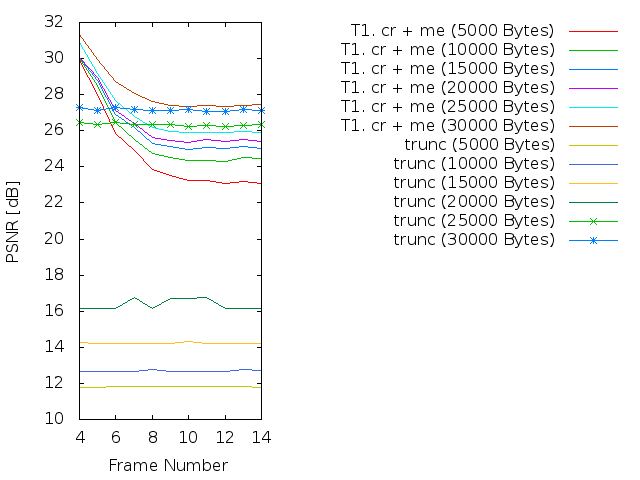
\includegraphics[width=0.5\textwidth]{benchmark/01_type1/psnr_type1.pdf}}
\caption{PSNR. Type 1}
\label{fig:image1}
\end{figure}

\begin{figure}[h!]
\centering
\resizebox{0.8\textwidth}{!}{
%\input{benchmark/01_type1/psnr_type1}}
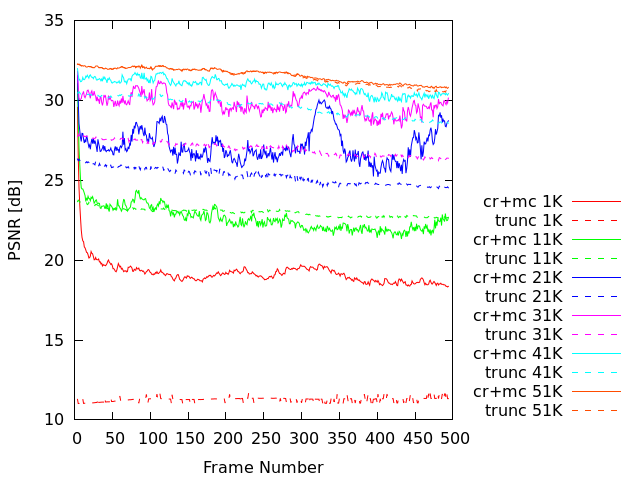
\includegraphics[width=0.5\textwidth]{benchmark/02_type2/psnr_type2.pdf}}
\caption{PSNR. Type 2}
\label{fig:image2}
\end{figure}

\begin{figure}[h!]
\centering
\resizebox{0.8\textwidth}{!}{
%\input{benchmark/01_type1/psnr_type1}}
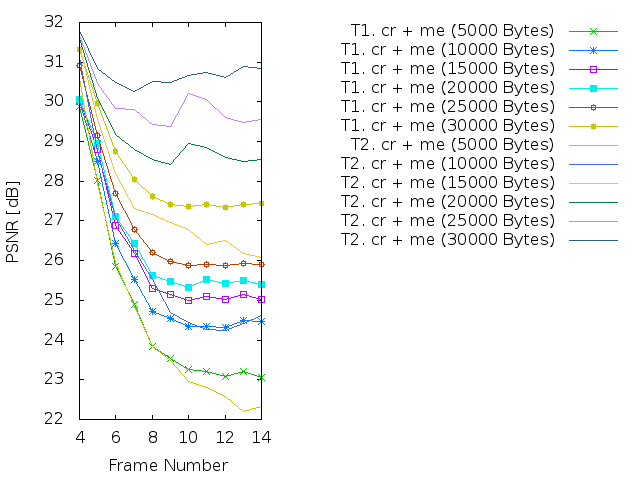
\includegraphics[width=0.5\textwidth]{benchmark/03_type1_vs_type2/psnr_type1_vs_type2.pdf}}
\caption{PSNR. Type1 vs Type 2}
\label{fig:image3}
\end{figure}


\section{Formato .j2c.cache}

Estamos utilizando un formato interno para trabajar con los precintos/paquetes del
codestream.

La estructura de los paquetes que se almacenan en los archivos \textbf{.j2c.cache} es la siguiente:
  
\begin{verbatim}  
--------------------------------------------------------------------
| precinct id (4 bytes) | l (4 bytes)  | r (4 bytes) | c (4 bytes) |
--------------------------------------------------------------------
| py (4 bytes)          | px (4 bytes) | packet length (4 bytes)   | 
--------------------------------------------------------------------
| packet                                                           |
--------------------------------------------------------------------
\end{verbatim}

\section{Cookcache}

Este programa recibe dos archivos con formato \textbf{.j2c.cache} y devuelve como salida
otro archivo con formato \textbf{.j2c.cache} formado por los paquetes vac\'ios necesarios
para completar los precintos que aparecen en el archivo \texttt{<response.j2c.cache>}. \\

{\color{blue}\texttt{cookcache <full.j2c.cache> <response.j2c.cache>}} \\

\textbf{Entrada:}

\begin{itemize}
\item \texttt{<full.j2c.cache>}: Este archivo contiene todo el codestream completo de una imagen.
\item \texttt{<response.j2c.cache>}: Este archivo contiene la respuesta que nos env\'ia el servidor,
para una petici\'on formada por una serie de WOIs (precintos) y un determinado bitrate. Lo normal es que esta
respuesta contega solamente algunos de los paquetes que forman un precinto, por este motivo habr\'a que
localizar cu\'ales son los paquetes que faltan para completar el precinto completo y crear paquetes
vac\'ios en su lugar.
\end{itemize}

\textbf{Salida:} \\

Este programa devuelve el archivo \texttt{emptypackets.j2c.cache} con todos los paquetes vac\'ios
que son necesarios para completar todos los precinctos.

La fusi\'on de los archivos \texttt{<response.j2c.cache>} + \texttt{emptypackets.j2c.cache} contendr\'a
el codestream necesario para poder realizar la fusi\'on de dos im\'agenes en el dominio JPEG2000.

\section{Paquetes vac\'ios}

Los paquetes vac\'ios que se han creado contienen 8 bytes y tienen el siguiente formato:

\begin{verbatim}  
 FF 91   00 04   XX XX   80 00
\_____/ \_____/ \_____/ \_____/
  SOP    Lsop    Nsop    Packet Body
\end{verbatim}

  \begin{itemize}
    \item \textbf{SOP}: Start of packet.
    \item \textbf{Lsop}: Length of marker segment in bytes (not including the marker).
    \item \textbf{Nsop}: Packet id [0..65535].
    \item \textbf{Packet Body}: Code-stream.
  \end{itemize}


  \begin{itemize}
    \item \texttt{$FF_{(16)}$ = unsigned char sop\_0 = $255_{(10)}$}.
    \item \texttt{$91_{(16)}$ = unsigned char sop\_1 = $145_{(10)}$}.
    \item \texttt{$00_{(16)}$ = unsigned char lsop\_0 = $0_{(10)}$}.
    \item \texttt{$04_{(16)}$ = unsigned char lsop\_1 = $4_{(10)}$}.
    \item \texttt{XX XX} se corresponde con el id del paquete.
    \item \texttt{$80_{(16)}$ = unsigned char body\_0 = $128_{(10)}$}.
    \item \texttt{$00_{(16)}$ = unsigned char body\_1 = $0_{(10)}$}.
  \end{itemize}

\section{Nuevo tama\~no de bloque para la lectura de paquetes}

Se ha modificado el tama\~no de la estructura que utiliz\'abamos para leer los paquetes de 
los archivos \texttt{.j2c} para luego almacenarlos en nuestro formato interno \texttt{.j2c.cache}. 
Por ejemplo en la aplicaci\'on \texttt{woistocache} los paquetes se le\'ian en bloques de $500$ bytes 
utilizando la estructura \texttt{kdu\_byte data$[500]$}. De modo que para un paquete de $2214$ bytes 
tendr\'iamos $5$ bloques en nuestro archivo \texttt{.j2c.cache}.

\begin{verbatim}
precinct.id = 176: 7 2 0 5 6: 500 bytes
precinct.id = 176: 7 2 0 5 6: 500 bytes
precinct.id = 176: 7 2 0 5 6: 500 bytes
precinct.id = 176: 7 2 0 5 6: 500 bytes
precinct.id = 176: 7 2 0 5 6: 214 bytes
\end{verbatim}


Hemos aumentado el tama\~no de bloque y ahora utilizamos la estructura \texttt{kdu\_byte data$[524288]$}.
De este modo garatizamos que en nuestro archivo \texttt{.j2c.cache} vamos a tener el paquete en 
un s\'olo bloque. (\color{red}{Tengo que revisar cu\'al es el tama\~no m\'aximo que puede tener
un paquete})

\end{document}